% Figure 2: fixed-arm multilingual repair ledger and score effects.
% All result values and plot coordinates come from figure2_defs.tex, generated
% from the canonical table6_multilingual.tex by analysis/figure2.py.
\documentclass[border=1pt]{standalone}
\ifdefined\pdftrailerid\pdftrailerid{}\fi

\usepackage[T1]{fontenc}
\usepackage[tt=false,type1=true]{libertine}
\usepackage[libertine]{newtxmath}
\usepackage{tikz}
\usetikzlibrary{arrows.meta,shapes.geometric}

% Generated by analysis/figure2.py from tables/table7_multilingual_mechanism.tex.
% Do not edit: every printed result and marker coordinate comes from the
% canonical generated table.
\newcommand{\ChineseLabel}{Chinese}
\newcommand{\ChineseCorpus}{AI CUP}
\newcommand{\ChineseRows}{2,000}
\newcommand{\ChineseInvalid}{12.55}
\newcommand{\ChineseNaNet}{+395}
\newcommand{\ChineseSubstNet}{-264}
\newcommand{\ChineseWfDelta}{-0.0011}
\newcommand{\ChineseTupleDelta}{+0.0350}
\newcommand{\ChineseWfX}{14.0587}
\newcommand{\ChineseTupleX}{17.0550}
\newcommand{\EnglishLabel}{English}
\newcommand{\EnglishCorpus}{ML-Promise}
\newcommand{\EnglishRows}{400}
\newcommand{\EnglishInvalid}{23.17}
\newcommand{\EnglishNaNet}{+148}
\newcommand{\EnglishSubstNet}{-86}
\newcommand{\EnglishWfDelta}{+0.0032}
\newcommand{\EnglishTupleDelta}{+0.0725}
\newcommand{\EnglishWfX}{14.4156}
\newcommand{\EnglishTupleX}{20.1675}
\newcommand{\FrenchLabel}{French}
\newcommand{\FrenchCorpus}{ML-Promise}
\newcommand{\FrenchRows}{400}
\newcommand{\FrenchInvalid}{21.08}
\newcommand{\FrenchNaNet}{+150}
\newcommand{\FrenchSubstNet}{-107}
\newcommand{\FrenchWfDelta}{+0.0036}
\newcommand{\FrenchTupleDelta}{+0.0625}
\newcommand{\FrenchWfX}{14.4488}
\newcommand{\FrenchTupleX}{19.3375}
\newcommand{\JapaneseLabel}{Japanese}
\newcommand{\JapaneseCorpus}{ML-Promise}
\newcommand{\JapaneseRows}{400}
\newcommand{\JapaneseInvalid}{31.25}
\newcommand{\JapaneseNaNet}{+183}
\newcommand{\JapaneseSubstNet}{-245}
\newcommand{\JapaneseWfDelta}{-0.0131}
\newcommand{\JapaneseTupleDelta}{+0.0708}
\newcommand{\JapaneseWfX}{13.0627}
\newcommand{\JapaneseTupleX}{20.0264}
\newcommand{\KoreanLabel}{Korean}
\newcommand{\KoreanCorpus}{ML-Promise}
\newcommand{\KoreanRows}{500}
\newcommand{\KoreanInvalid}{22.73}
\newcommand{\KoreanNaNet}{+103}
\newcommand{\KoreanSubstNet}{-148}
\newcommand{\KoreanWfDelta}{-0.0192}
\newcommand{\KoreanTupleDelta}{+0.0293}
\newcommand{\KoreanWfX}{12.5564}
\newcommand{\KoreanTupleX}{16.5819}
\newcommand{\LanguageCount}{5}
\newcommand{\TuplePositiveCount}{5}
\newcommand{\WfPositiveCount}{2}


\definecolor{ink}{HTML}{273746}
\definecolor{muted}{HTML}{64727D}
\definecolor{panelgrey}{HTML}{F6F7F8}
\definecolor{blue}{HTML}{0072B2}
\definecolor{bluefill}{HTML}{DCEEF8}
\definecolor{teal}{HTML}{009E73}
\definecolor{tealfill}{HTML}{DDF2EB}
\definecolor{vermillion}{HTML}{D55E00}
\definecolor{vermillionfill}{HTML}{F9E6DC}
\definecolor{purple}{HTML}{8B6BB1}
\definecolor{purplefill}{HTML}{EEE8F5}

\tikzset{
  panel/.style={rounded corners=5pt, draw=muted!42, fill=panelgrey,
                line width=0.38pt},
  header/.style={anchor=west, text=white, font=\bfseries\small},
  subheader/.style={anchor=west, text=muted, font=\bfseries\scriptsize},
  language/.style={anchor=west, text=ink, font=\bfseries\footnotesize,
                   align=left},
  invalid/.style={rounded corners=4pt, draw=vermillion,
                  fill=vermillionfill, text=vermillion!75!black,
                  line width=0.45pt, font=\scriptsize, align=center,
                  minimum width=1.55cm, inner ysep=2pt},
  projection/.style={rounded corners=4pt, draw=blue, fill=bluefill,
                     text=blue!75!black, line width=0.45pt,
                     font=\bfseries\scriptsize, inner xsep=3pt,
                     inner ysep=2pt},
  positive/.style={rounded corners=4pt, draw=teal, fill=tealfill,
                   text=teal!70!black, line width=0.45pt,
                   font=\scriptsize, align=center, minimum width=1.25cm,
                   inner ysep=2pt},
  negative/.style={rounded corners=4pt, draw=vermillion,
                   fill=vermillionfill, text=vermillion!75!black,
                   line width=0.45pt, font=\scriptsize, align=center,
                   minimum width=1.65cm, inner ysep=2pt},
  guide/.style={draw=muted!26, line width=0.35pt},
  value/.style={font=\tiny, inner sep=1pt},
  flow/.style={draw=muted!72, line width=0.42pt,
               -{Stealth[length=2.7pt,width=2.2pt]}},
}

% One language row on the repair-ledger side. Cards carry exact signed counts;
% their equal widths are intentional because corpus sizes differ.
\newcommand{\ledgerrow}[7]{%
  \node[language] at (0.25,#7)
    {#1\\[-1pt]\normalfont\tiny #2\\[-1pt]#3 rows};
  \draw[flow] (3.95,#7) -- (4.52,#7);
  \draw[flow] (5.76,#7) -- (6.30,#7);
  \node[invalid] at (3.15,#7) {M0 #4\%\\invalid};
  \node[projection] at (5.15,#7) {project};
  \node[positive] at (7.05,#7) {$N\!/\!A$\\\textbf{#5}};
  \node[negative] at (9.45,#7) {substantive\\\textbf{#6}};
}

% A circle and a diamond remain distinct if the page is printed in greyscale.
\newcommand{\deltarow}[5]{%
  \pgfmathsetmacro{\wfY}{#5+0.17}
  \pgfmathsetmacro{\tupleY}{#5-0.17}
  \filldraw[fill=vermillion, draw=white, line width=0.35pt]
    (#1,\wfY) circle (2.25pt);
  \node[value, text=vermillion!80!black, anchor=south]
    at (#1,{\wfY+0.08}) {#3};
  \node[diamond, draw=teal, fill=teal, minimum size=4.8pt, inner sep=0pt]
    at (#2,\tupleY) {};
  \node[value, text=teal!70!black, anchor=north]
    at (#2,{\tupleY-0.08}) {#4};
}

\begin{document}
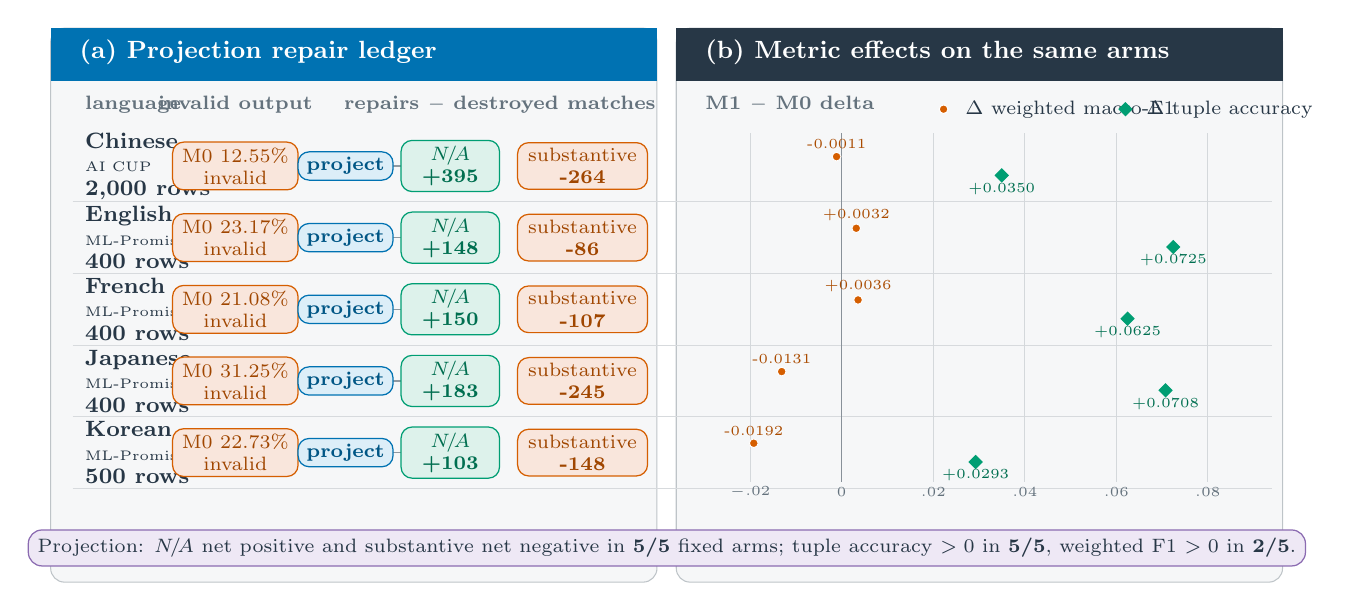
\begin{tikzpicture}[scale=0.70, font=\footnotesize]
  \filldraw[panel] (-0.2,0.2) rectangle (10.8,10.25);
  \filldraw[panel] (11.15,0.2) rectangle (22.15,10.25);
  \fill[blue] (-0.2,9.3) rectangle (10.8,10.25);
  \fill[ink] (11.15,9.3) rectangle (22.15,10.25);
  \node[header] at (0.15,9.82) {(a) Projection repair ledger};
  \node[header] at (11.5,9.82) {(b) Metric effects on the same arms};

  \node[subheader] at (0.25,8.87) {language};
  \node[subheader, anchor=center] at (3.15,8.87) {invalid output};
  \node[subheader, anchor=center] at (7.95,8.87) {repairs $-$ destroyed matches};
  \node[subheader] at (11.5,8.87) {M1 $-$ M0 delta};

  \foreach \rowY in {7.75,6.45,5.15,3.85,2.55}
    \draw[guide] (0.2,{\rowY-0.65}) -- (21.95,{\rowY-0.65});

  \ledgerrow{\ChineseLabel}{\ChineseCorpus}{\ChineseRows}
    {\ChineseInvalid}{\ChineseNaNet}{\ChineseSubstNet}{7.75}
  \ledgerrow{\EnglishLabel}{\EnglishCorpus}{\EnglishRows}
    {\EnglishInvalid}{\EnglishNaNet}{\EnglishSubstNet}{6.45}
  \ledgerrow{\FrenchLabel}{\FrenchCorpus}{\FrenchRows}
    {\FrenchInvalid}{\FrenchNaNet}{\FrenchSubstNet}{5.15}
  \ledgerrow{\JapaneseLabel}{\JapaneseCorpus}{\JapaneseRows}
    {\JapaneseInvalid}{\JapaneseNaNet}{\JapaneseSubstNet}{3.85}
  \ledgerrow{\KoreanLabel}{\KoreanCorpus}{\KoreanRows}
    {\KoreanInvalid}{\KoreanNaNet}{\KoreanSubstNet}{2.55}

  % Common delta axis: -0.02 to +0.08, with zero emphasised.
  \foreach \x/\tick in {12.49/$-.02$,14.15/$0$,15.81/$.02$,
                         17.47/$.04$,19.13/$.06$,20.79/$.08$} {
    \draw[draw=muted!28, line width=0.35pt] (\x,2.02) -- (\x,8.35);
    \node[font=\tiny, text=muted] at (\x,1.83) {\tick};
  }
  \draw[draw=ink!55, line width=0.62pt] (14.15,2.02) -- (14.15,8.35);

  \deltarow{\ChineseWfX}{\ChineseTupleX}
    {\ChineseWfDelta}{\ChineseTupleDelta}{7.75}
  \deltarow{\EnglishWfX}{\EnglishTupleX}
    {\EnglishWfDelta}{\EnglishTupleDelta}{6.45}
  \deltarow{\FrenchWfX}{\FrenchTupleX}
    {\FrenchWfDelta}{\FrenchTupleDelta}{5.15}
  \deltarow{\JapaneseWfX}{\JapaneseTupleX}
    {\JapaneseWfDelta}{\JapaneseTupleDelta}{3.85}
  \deltarow{\KoreanWfX}{\KoreanTupleX}
    {\KoreanWfDelta}{\KoreanTupleDelta}{2.55}

  \filldraw[fill=vermillion, draw=white] (16.0,8.78) circle (2.25pt);
  \node[font=\scriptsize, anchor=west, text=ink] at (16.22,8.78)
    {$\Delta$ weighted macro-F1};
  \node[diamond, draw=teal, fill=teal, minimum size=4.8pt, inner sep=0pt]
    at (19.3,8.78) {};
  \node[font=\scriptsize, anchor=west, text=ink] at (19.5,8.78)
    {$\Delta$ tuple accuracy};

  \node[rounded corners=5pt, draw=purple, fill=purplefill,
        line width=0.45pt, text=ink, font=\scriptsize,
        minimum width=14.6cm, inner ysep=3pt] at (10.98,0.82)
    {Projection: $N\!/\!A$ net positive and substantive net negative in
     \textbf{\LanguageCount/\LanguageCount} fixed arms; tuple accuracy
     $>0$ in \textbf{\TuplePositiveCount/\LanguageCount}, weighted F1
     $>0$ in \textbf{\WfPositiveCount/\LanguageCount}.};
\end{tikzpicture}
\end{document}
